\pagebreak
\subsection{SiPm}
Il rilevatore presenta al suo interno il sistema composto da SPAD e resistenze di quenching che permette la creazione di valanghe di elettroni controllate all'interno del rilevatore fino ad ottenere una risoluzione al singolo fotone.

\subsubsection{Setup}

Siccome la tensione generata dal SiPm è troppo bassa per la risoluzione dell'ADC è necessario applicare gli stadi di amplificazione studiati nei punti seguenti come mostrato in figura:

\begin{figure}[!h]
    \centering
    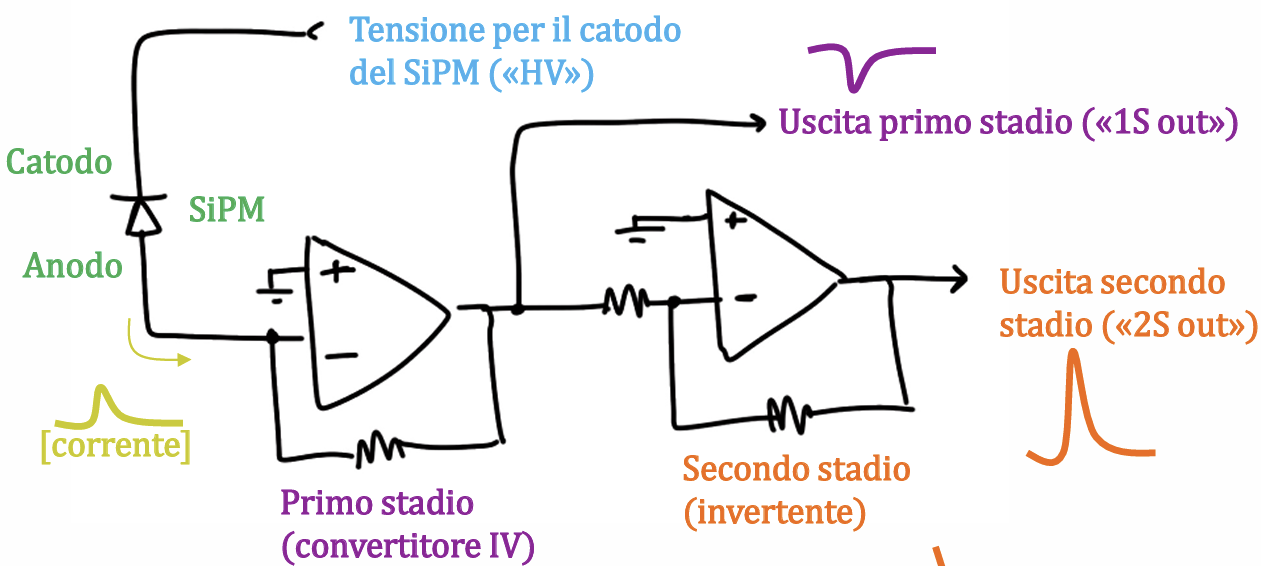
\includegraphics[width=0.5\linewidth]{Photomultiplier/assets/SiPm/SiPm_Stadi_Amp.png}
    \caption{Stadi di amplificazione}
    \label{fig:SiPm stadi di amp}
\end{figure}

Siccome i tempi di esistenza del segnale sono molto bassi, nell'ordine dei 100-200ns, risulta difficile ottenere una misurazione accurata con l'ADC che è limitato a campionamenti nell'ordine dei 300ns. Per questo è stato usato un sistema di Peak Hold:

\begin{figure}[!h]
    \centering
    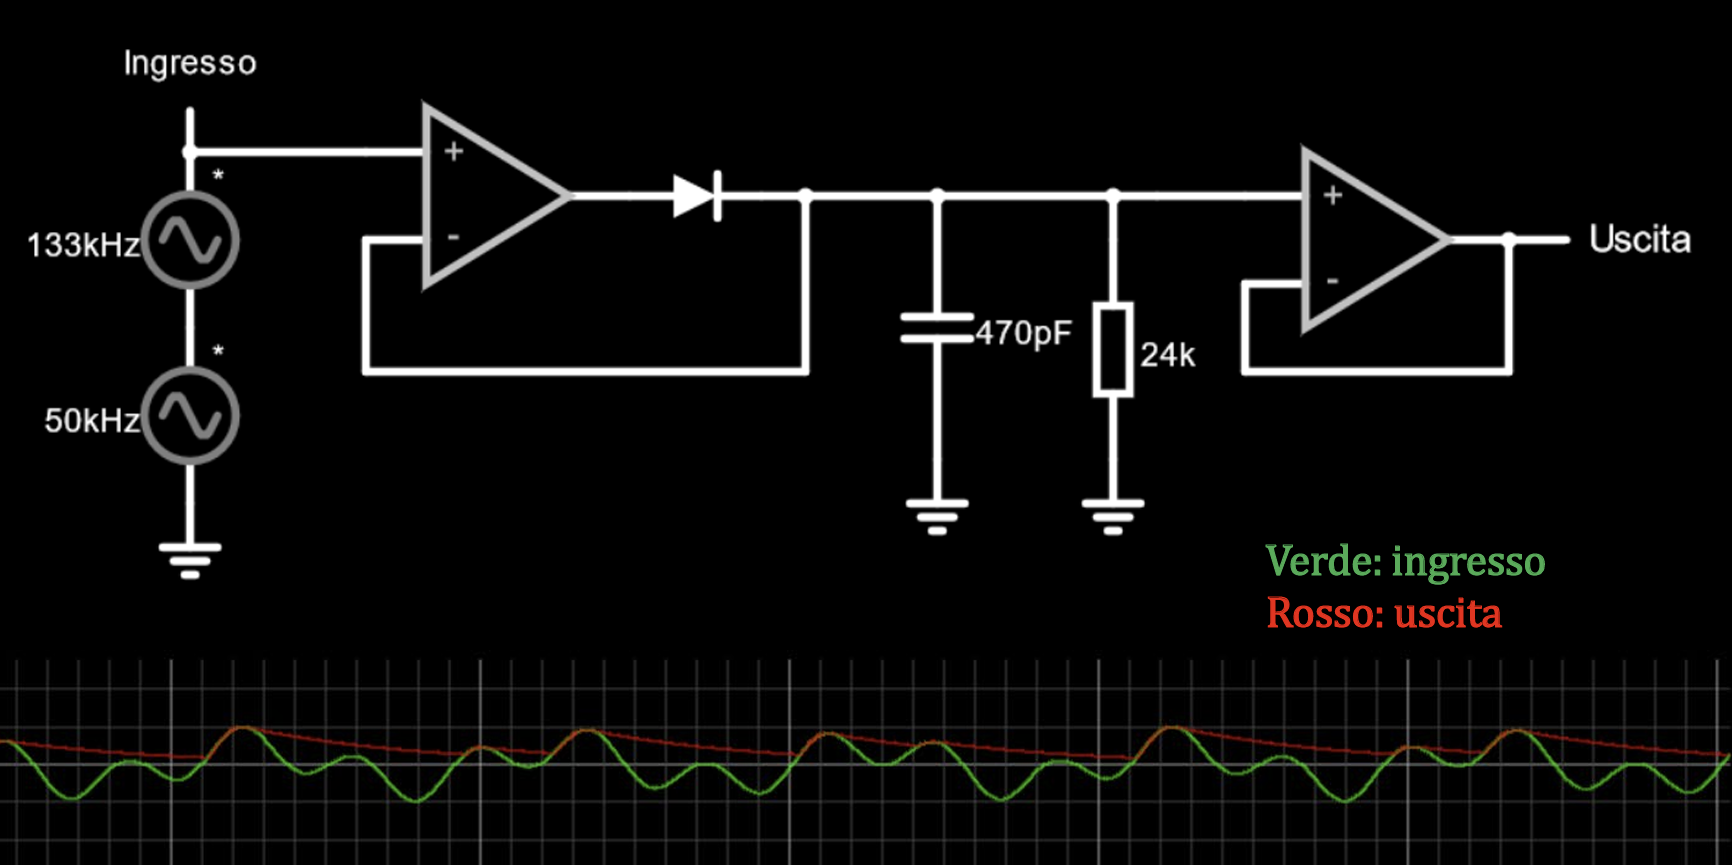
\includegraphics[width=0.5\linewidth]{Photomultiplier/assets/SiPm/SiPm_Peak_hold.png}
    \caption{Sistema di Peak Hold}
\end{figure}

All'uscita del peak hold la tensione viene mantenuta per un tempo sufficiente per l'acquisizione dell'ADC.

Per comprendere la polarizzazione, è stata impostata inizialmente sull'alimentatore una tensione bassa e corrente limitata per controllare la polarizzazione corretta. Avendo inserito nei suoi pin la fonte luminosa a LED, è stata sigillata la zona contenente fonte luminosa e rilevatore. Successivamente, la tensione fornita al SiPm è stata portata a +3V di Overvoltage per permettere l'avvento della valanga di elettroni nello SPAD.

Fornendo al LED una tensione impulsata di 100 ns a circa 3.4 V è stato possibile osservare la rilevazione dei fotoni:

\begin{figure}[!h]
    \centering
    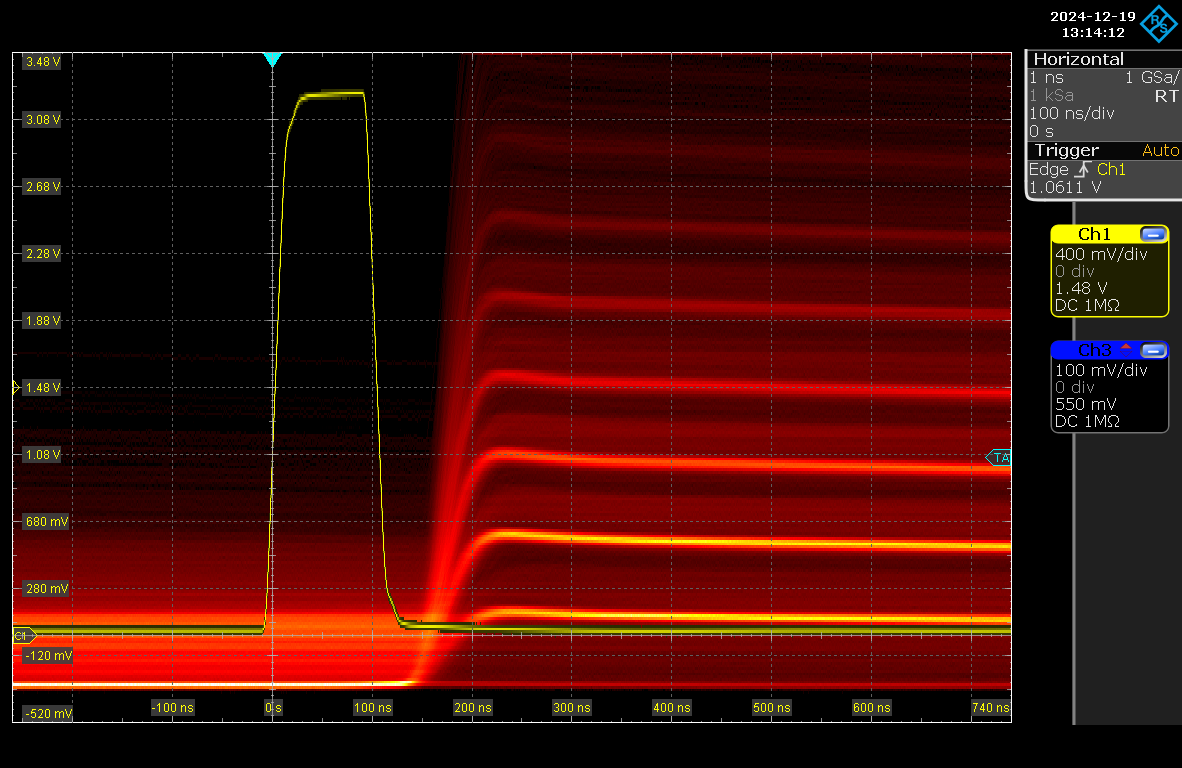
\includegraphics[width=0.5\linewidth]{Photomultiplier/assets/SiPm/SiPm.png}
    \caption{Prima visualizzazione dei segnali con persistance di 2 sec}
\end{figure}

E evidente la presenza di diverse zone con elevata densità di rilevazioni
che corrispondono a 1 fotone, 2 fotoni, 3 fotoni etc...

\subsubsection{Dark Count Rate}
Siccome gli elettroni nello spad sono soggetti ad agitazione termica, è possibile che un elettrone riesca casualmente a liberarsi anche senza la presenza di un fotone, portando a una valanga non desiderata. Questo è noto come DCR (Dark Count Rate).

Per caratterizzare il SiPm è utile avere una stima di questo fenomeno. Per questo è stato impostato l'oscilloscopio in modalità di conteggio dei segnali in arrivo. Impostata una soglia di trigger di circa mezzo fotone è stata fatta partire la misura di tempo per 40000 segnali a tensioni di overvoltage differenti.

\begin{figure}[!h]
    \centering
    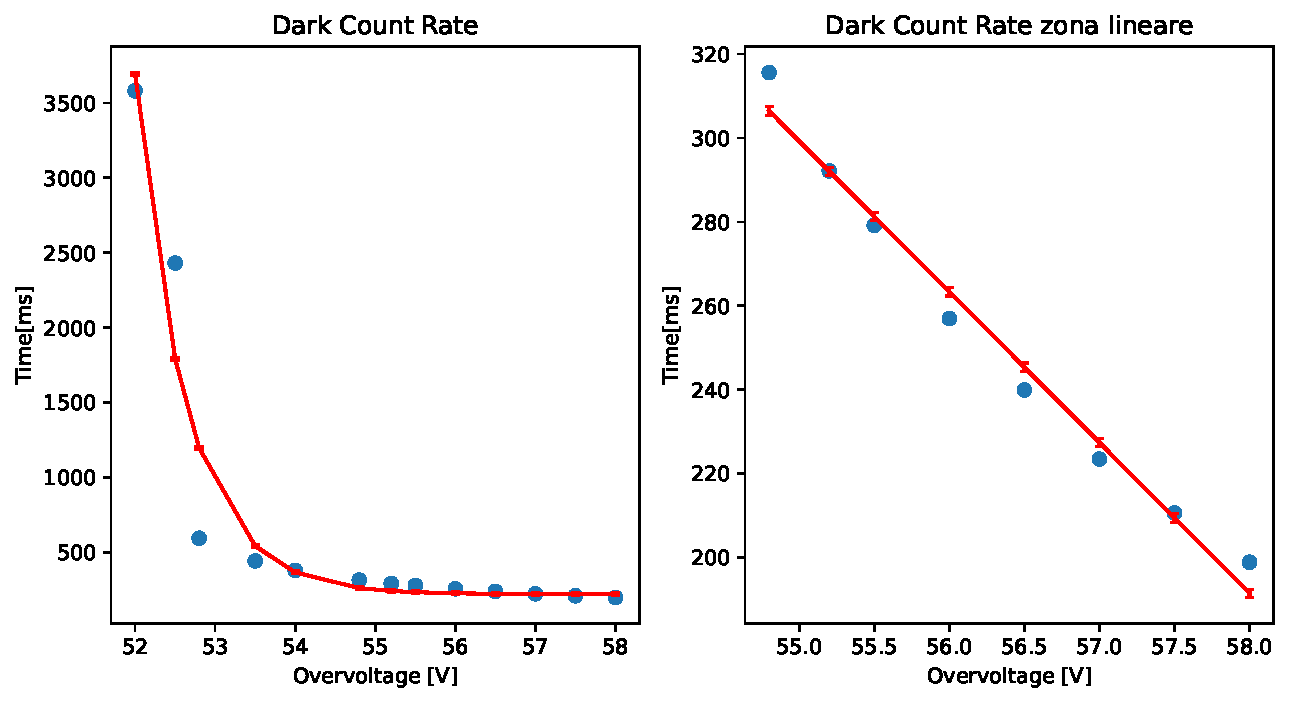
\includegraphics[width=0.6\linewidth]{Photomultiplier/assets/SiPm/SiPm_DCR.pdf}
    \caption{Tempi per conteggio di 40000 eventi, (\href{https://github.com/Yedi278/Esperimentazioni-Elettronica/tree/main/SiPm/Caratterizzazione\%20Hamamatsu}{link dati})}
\end{figure}

Nella zona prossima alla tensione di \textit{break down} il rate risulta molto basso, si suppone dovuto alla mancanza di campo elettrico fornito agli elettroni che non sono in grado in certi casi di produrre la valanga. Per tenisoni prossime a quelle di \textit{overvoltage} consigliate, ovvero $V_{OV} = 54.9V$, il rate si comporta in maniera approssimativamente lineare. Siccome il rate cambia di circa 31 ms/V possiamo approssimare questo rate ad un valore costante di circa \textbf{DCR = 158±38KHz}.
Questo valore risulta ragionevole con i valori inclusi nel manuale.